In this section we provide two different case studies involving a mars rover. In the first experiment the rover has to plan around a moving obstacle, but the knowledge of the location of the moving obstacle is penalized. In the second experiment, the rover has some a priori knowledge of the terrain, but there is a cost to using any additional information. 

\subsection{Moving obstacle}
We solve the motion planning problem under sensing constraints in a gridworld as shown in \ref{fig:casestudy}\subref{fig:exp1}. Consider a scenario where rover is tasked with reaching the goal state in green whilst avoiding collisions with the red static obstacles and an orange moving obstacle that moves in the area shown. For example, the helicopter can be completing a separate mission and we do not want the rover and helicopter to collide, but we also want to limit their communication to conserve power. Hence, we treat the helicopter as a moving obstacle and add an information cost to its position.

We express this in LTL as $\lnot$'crash' $\LTLuntil$ 'goal'. Where the atomic proposition 'crash' is true in the red static obstacles and when the state of the rover is the same as the state of the moving obstacle. The atomic proposition 'goal' is true in the green cell. The DFA representation is shown in Figure \ref{fig:casestudy}\subref{fig:dra}.
\begin{figure}
\subfloat[Gridworld with moving obstacle \label{fig:exp1}]{
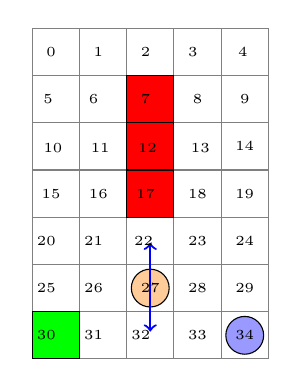
\begin{tikzpicture}[scale=1.2]
\draw[step=0.5cm,color=gray] (-1.5,-2.5) grid (1,1);
\filldraw[fill=red,draw=black] (0,0.5) rectangle (-0.5,0);
\filldraw[fill=red,draw=black] (0,0) rectangle (-0.5,-0.5);
\filldraw[fill=red,draw=black] (0,-0.5) rectangle (-0.5,-1);
\filldraw[fill=green,draw=black] (-1.5,-2.5) rectangle (-1,-2.0);
\filldraw[fill=blue!40!white,draw=black] (+0.75,-2.25) circle (0.2cm);
\filldraw[fill=orange!40!white,draw=black] (-0.25,-1.75) circle (0.2cm);
\draw[blue,thick,->] (-0.25,-1.73) -> (-0.25,-1.27);
\draw[blue,thick,->] (-0.25,-1.73) -> (-0.25,-2.21);
\node at (-1.30,+0.75) {\tiny{0}};
\node at (-0.80,+0.75) {\tiny{1}};
\node at (-0.30,+0.75) {\tiny{2}};
\node at (0.20,+0.75) {\tiny{3}};
\node at (0.73,+0.75) {\tiny{4}};
\node at (-1.33,+0.25) {\tiny{5}};
\node at (-0.85,+0.25) {\tiny{6}};
\node at (-0.3,+0.25) {\tiny{7}};
\node at (0.25,+0.25) {\tiny{8}};
\node at (0.75,+0.25) {\tiny{9}};
\node at (-1.28,-0.27) {\tiny{10}};
\node at (-0.78,-0.27) {\tiny{11}};
\node at (-0.28,-0.27) {\tiny{12}};
\node at (0.28,-0.27) {\tiny{13}};
\node at (0.75,-0.25) {\tiny{14}};
\node at (-1.3,-0.75) {\tiny{15}};
\node at (-0.8,-0.75) {\tiny{16}};
\node at (-0.3,-0.75) {\tiny{17}};
\node at (0.25,-0.75) {\tiny{18}};
\node at (0.75,-0.75) {\tiny{19}};
\node at (-1.35,-1.25) {\tiny{20}};
\node at (-0.85,-1.25) {\tiny{21}};
\node at (-0.32,-1.25) {\tiny{22}};
\node at (0.25,-1.25) {\tiny{23}};
\node at (0.75,-1.25) {\tiny{24}};
\node at (-1.35,-1.75) {\tiny{25}};
\node at (-0.85,-1.75) {\tiny{26}};
\node at (-0.25,-1.75) {\tiny{27}};
\node at (0.25,-1.75) {\tiny{28}};
\node at (0.75,-1.75) {\tiny{29}};
\node at (-1.35,-2.25) {\tiny{30}};
\node at (-0.85,-2.25) {\tiny{31}};
\node at (-0.35,-2.25) {\tiny{32}};
\node at (0.25,-2.25) {\tiny{33}};
\node at (0.75,-2.25) {\tiny{34}};
\end{tikzpicture}
}
\subfloat[Specification DFA\label{fig:dra}]{
	\begin{tikzpicture}[shorten >=1pt,node distance=1.6cm,on grid]
	\node[state,initial]   (q_0)                {$s_0$};
	\node[state,accepting]           (q_1) [right=of q_0] {$s_1$};
	\node[state] (q_2) [below=of q_1] {$s_2$};
	\path[->] (q_0) edge                node [above] {\small Goal} (q_1)
	edge [loop above]   node         {} ()
	%edge [bend left=45] node [below] {1} (q_2)
	edge [bend right]   node [left] {\small Crash} (q_2)
	(q_1) edge                node [right] {\small Crash} (q_2)
	edge [loop above]         node {} (q_1)
	(q_2) edge [loop below]   node {} (q_2);
	\end{tikzpicture}
}
\caption{Gridworld and DFA  with $\textrm{Acc}_{\mathcal{M}} = (s_1)$ depicting a scenario where agent in blue has to reach green target cell without crashing into the red static obstacles or the orange moving obstacle.}\label{fig:casestudy}
\end{figure}

The rover has the choice of moving in 4 directions - North, South, East, and West or staying still. The motion is stochastic - i.e, it has a probability of slip. For example, if it chooses to move north, it has a probability to 'slip' and move to a state north east or north west. 

The state space of the MDP is $(x,y,x_{obs},y_{obs})$ where $(x,y)$ is the position of the rover and $(x_{obs},y_{obs})$ is the position of the moving obstacle. We assume that the state of the moving obstacle to be expensive to observe. Formally, we let $\mathcal{\tilde{X}} = (x,y)$ and $\mathcal{\bar{X}} = (x_{obs},y_{obs})$. 

Since there is a probability to slip, the agent has a non-zero probability of crashing and not satisfying the specification if it goes the long way around the wall. If the agent knows the position of the moving obstacle at all times, it can plan to avoid collision, and hence the shorter path will have the higher probability of satisfaction. Intuitively we expect to see if that we set the $\beta$ parameter high, \ie if the cost of information is high, the agent will go the long way around the wall as it will be too expensive to observe the moving obstacle. We use a time horizon $T = 25$ and test for $\beta = 0.5$ and $\beta=5$

\begin{figure}
	\subfloat[$\beta = 0.5$\label{simple-grid}]{
	\includegraphics[scale=.5]{lowbb}}
	%\hfill
	\subfloat[$\beta = 5$\label{fig:simple-transitions}]{
		\includegraphics[scale=0.5]{highb}
	}
	\caption{Probability distribution of the agent after 16/25 timesteps. a) has a low $\beta$ which means information cost is low while b) has a high $\beta$ and hence high cost on information}
	\label{fig:expres}
\end{figure}

Figure \ref{fig:expres} shows the probability distributions of the agent at a specific time $t=16$. Clearly, in the case where $\beta=0.5$, the agent is able to go through the region where the moving obstacle operates. However, when we increase the cost of information, the agent moves around the static obstacles.

\subsection{Static obstacles}\label{sec:marsexp}
Now, we present the example of the Mars rover navigating in the presence of static obstacles. Figure \ref{fig:mars} shows an example of a simple map of the environment that can obtained from a satellite image. This gives us a rough knowledge of the environment. We know the red region is impassable terrain. We also know that there is a region with a high density of obstacles and one with a low density of obstacles. All other regions are assumed to be obstacle free.

\begin{figure}
\centering
\begin{minipage}{5.0cm}
\subfloat[Simple martian environment for case study. The red region is already known as impassable terrain. Additionally, two areas are identified as having a high and low probability of obstacles respectively\label{fig:mars}]{
	\includegraphics[scale=0.1]{casestudygrid.png}
}
\end{minipage}

\begin{minipage}{5.0cm}
\subfloat[True obstacle distribution of the scenario from \ref{fig:mars}. Red cells are obstacles, and the green cells represent the target region the rover shown in blue is trying to reach. \label{fig:mars_grid}]{
	\includegraphics[scale=0.35]{casestudygrid_sim.png}
}
\end{minipage}
\caption{We represent the environment in \ref{fig:mars} as a gridworld in \ref{fig:mars_grid} which we model as an MDP. 
	}
\end{figure}

The LTL specification is again $\lnot$'crash' $\LTLuntil$ 'goal' where the goal is the green region. This time the state in the MDP is given by $(x,y,(o_1,\dots,o_n))$ where $o_i \in [0,1]$ are probability values indicating the likelihood there is an obstacle in state $(x_i,y_i)$. We assign discrete values to $o_i$ by constraining it to values in the set $o_i \in [0,0.2,0.4,0.6,0.8,1]$. 

We model the helicopter flying ahead and scouting by allowing $o_i$ to transition to $0$ or $1$ with probability given by the value of $o_1$ if the rover is within distance $d$ of the obstacle. More explicitly, the state $(x_i,y_i,(o_1,\dots,o_j,\dots,o_n))$ will transition to $(x_i,y_i,(o_1,\dots,1,\dots,o_n))$ with probability $o_j$ and transition to $(x_i,y_i,(o_1,\dots,0,\dots,o_n))$ with probability $1 - o_j$. This will only happen if distance between the states $(x_i,y_i)$ and $(x_j,y_j)$ is less than or equal to $d$. $o_i = 1$ indicates there is an obstacle present in $(x_i,y_i)$. 

The region with sparse obstacle distribution has mostly $o_i = 0$ while the dense obstacle region has many more states with $o_i > 0$. Intuitively this means that the rover will need the helicopter to scout ahead more often in the route with more obstacles. We assign the transfer entropy cost to states $(o_1,\dots o_n)$ which will penalize using these states in the policy synthesis.

\begin{figure}
	\begin{minipage}{5.0cm}
		\centering
		\subfloat[$t = 10$ \label{fig:casefine1t2}]{
			\includegraphics[scale=0.15]{casestudygrid_sim.png}\hspace{.5cm}
		}
		\subfloat[$t = 20$ \label{fig:case1finet3}]{
			\includegraphics[scale=0.15]{casestudygrid_sim.png}\hspace{.5cm}
		}
		\subfloat[$t= 30$ \label{fig:case1finet4}]{
			\includegraphics[scale=0.15]{casestudygrid_sim.png}\hspace{.5cm}
		}
	\end{minipage}
	\begin{minipage}{5.0cm}
		\centering
		\subfloat[$t = 10$  \label{fig:case1finet5}]{
			\includegraphics[scale=0.15]{casestudygrid_sim.png}\hspace{.5cm}
		}
		\subfloat[$t = 20$ \label{fig:case1finet6}]{
			\includegraphics[scale=0.15]{casestudygrid_sim.png}\hspace{.5cm}
		}
		\subfloat[$ = 30$ \label{fig:case1finet7}]{
			\includegraphics[scale=0.15]{casestudygrid_sim.png}\hspace{.5cm}
		}
		
	\end{minipage}
	
	
	\caption{Probability distribution of the rover location over time for two cases: (a) - (c) : $\beta = 0$, (d) - (f): $\beta = 10$. \textbf{Will add results}
	}
	\label{fig:marsresults}
\end{figure}


Figure \ref{fig:marsresults} shows the evolution of the probability distribution of the agent when the information is free (i.e $\beta$ is small) and when information is expensive ($\beta$ is large). We see that when information is free, the rover takes the path through the dense obstacle distribution. Also note that since there is no information cost, the problem reduces to solving pure reachability and the policy is deterministic. When we set $\beta = 10$, the rover takes the path through the sparse obstacle region.
